\section{Virtual Machine}
Hypotetische Maschine mit virtuellem Prozessor
\begin{itemize}
    \item Eigener Instruktionssatz: Intermediate Language
    \item Hülle um den realen Prozessor
\end{itemize}
\textbf{Nutzen:}
\begin{itemize}
    \item Mehrplattformen
    \item Mehrsprachigkeit
    \item Sicherheit
\end{itemize}

\subsection{Loader}
\begin{itemize}
    \item Lädt Zwischencode (File) in Speicher
    \item Alloziert Speicher (Metadaten für Klassen, Methoden, Variablen, Code)
    \item Definiert Layouts (Speicherbereiche für Fields/Variablen/Parameter)
    \item Address Relocation
    \begin{itemize}
        \item Löst Verweise auf zu Methoden, Typen, andere Assemblies
    \end{itemize}
    \item Initiiert Programmausführung
    \item Optional: Verifier
\end{itemize}

\subsubsection{Verifier}
\textbf{Erkenne und verhindere falscher IL-Code}
\begin{itemize}
    \item Statische Analyse zur Ladezeit
    \item Fehler in Compuler, böswillige Manipulationen
\end{itemize}
\textbf{Denkbare Fehler}
\begin{itemize}
    \item Typfehler
    \item Stack-Überlauf oder Unterlauf
    \item Nicht definierte Variablen/Methoden/Klassen
    \item Illegale Sprünge
\end{itemize}
\textbf{Alternative: Überprüfung zur Laufzeit}

\subsubsection{Metadaten}
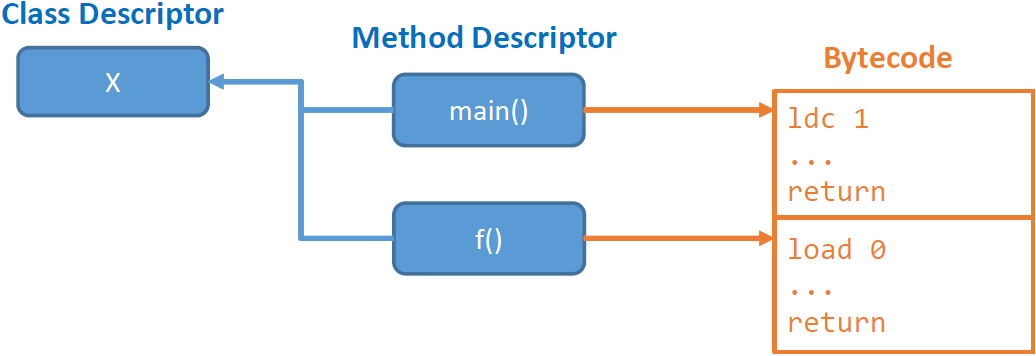
\includegraphics[width=0.5\linewidth]{metadaten.png}

\subsubsection{Deskriptoren}
\textbf{Laufzeitinfo für Typen \& Methoden}
\begin{itemize}
    \item Typen: Klassen, Arrays oder Basistypen
    \item Klassen: Field-Typen
    \item Methoden: Typen von Parameter \& Locals, Rückgabetyp, Bytecode
    \item Zusätzlich bei Klassen: Parent-Klasse, virtual Method Table
\end{itemize}
\vspace{0.5cm}
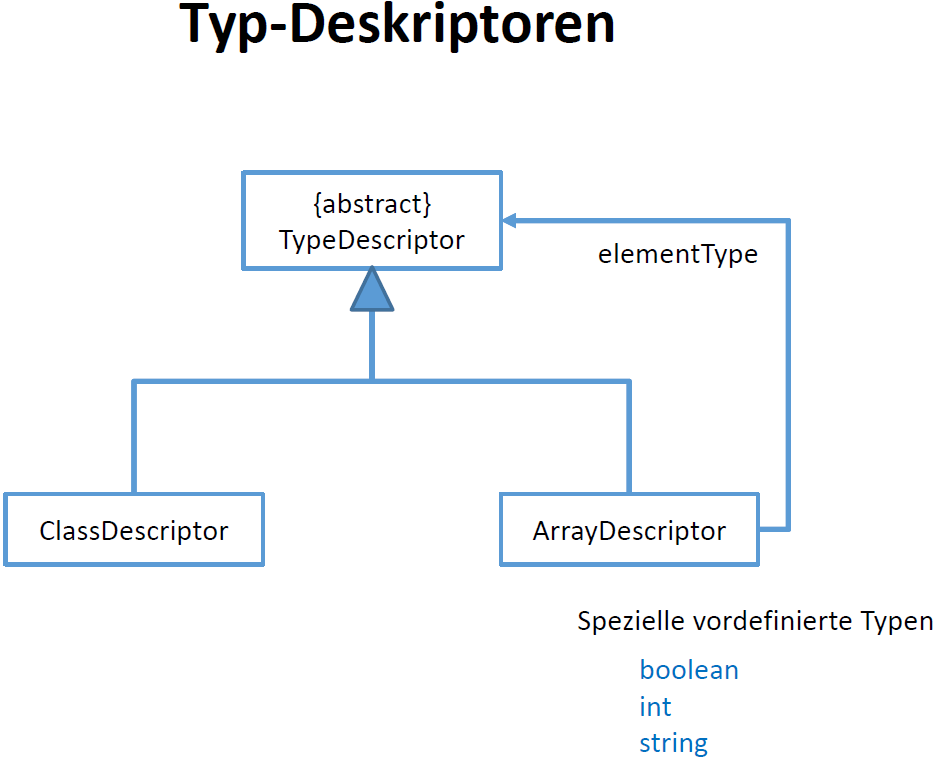
\includegraphics[width=0.5\linewidth]{typ_deskriptoren.png}
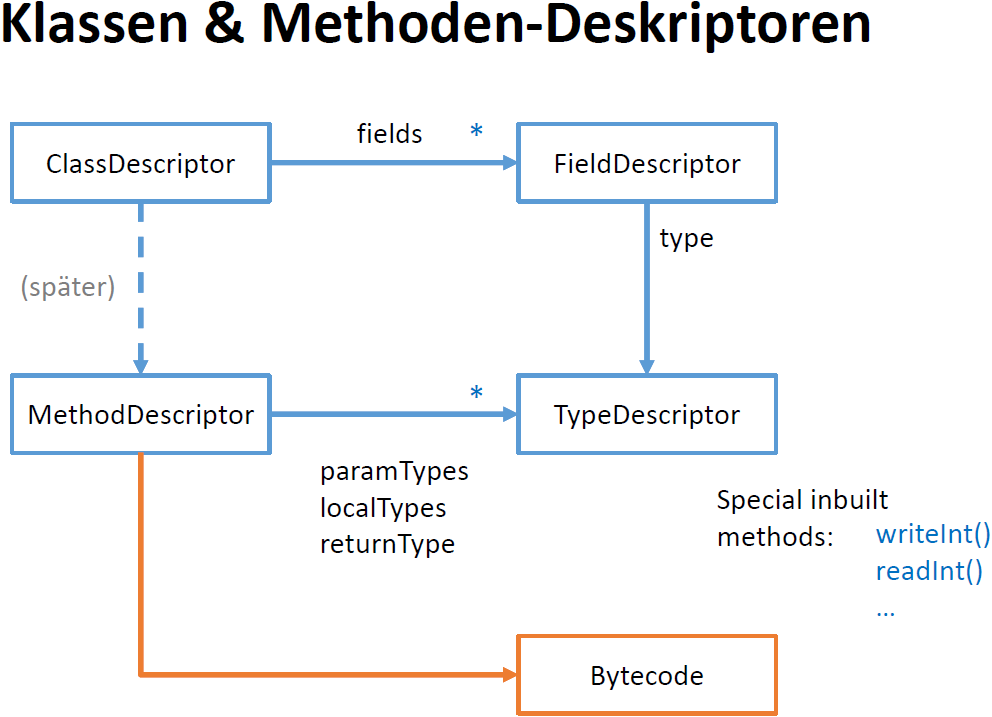
\includegraphics[width=0.5\linewidth]{klassen_deskriptoren.png}

\subsubsection{Bytecode Loading}
\begin{itemize}
    \item Von File direkt in Speicher geladen
    \item \textbf{Patching/Fixup:} Argumente in Instruktion anpassen
    \item Referenzen auf entsprechende Metadaten
\end{itemize}
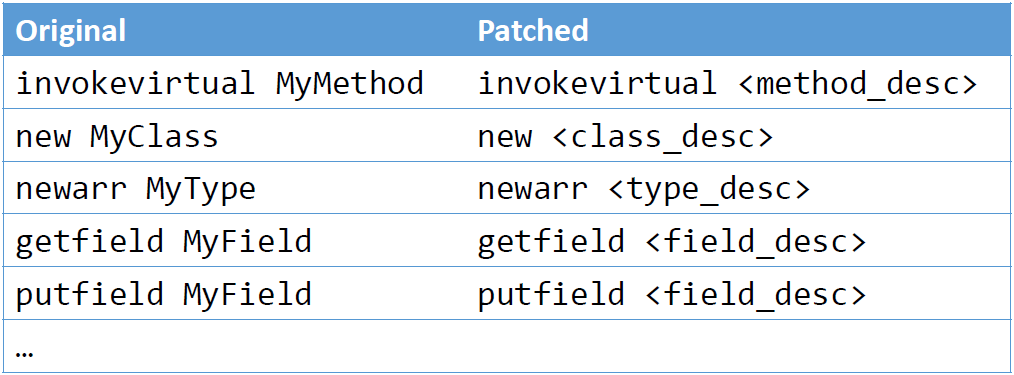
\includegraphics[width=0.5\linewidth]{patching.png}
\subsubsection{Patching}
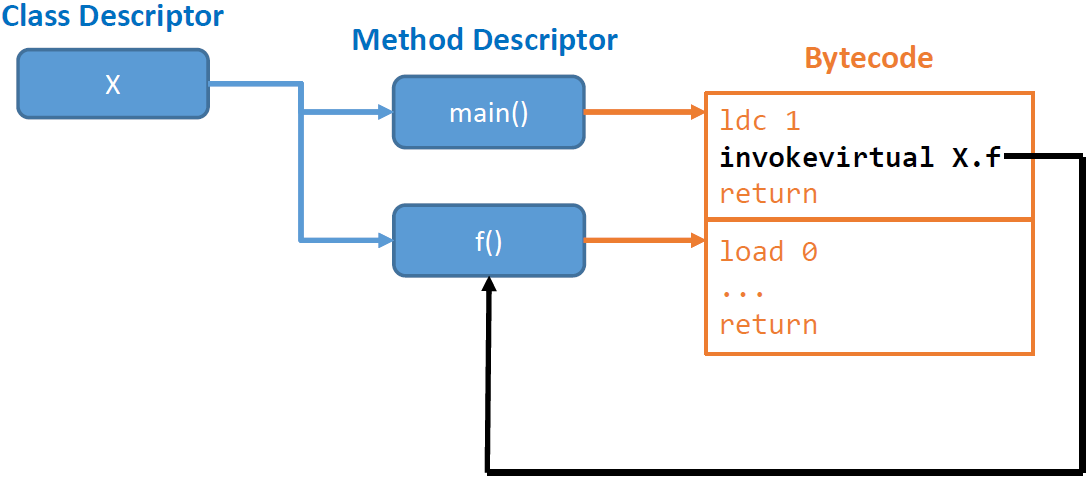
\includegraphics[width=0.5\linewidth]{patching2.png}

\subsubsection{VM: Managed \& Unmanaged}
\textbf{Kleine Unmanaged Teile neben der Java VM}
\begin{itemize}
    \item Heap und HW-Excution (JIT)
\end{itemize}
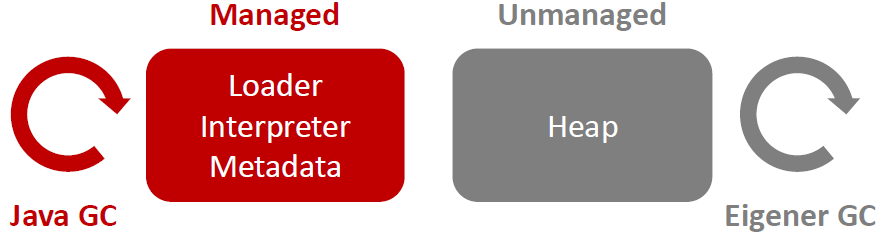
\includegraphics[width=0.5\linewidth]{managed.png}

\subsection{Interpreter}
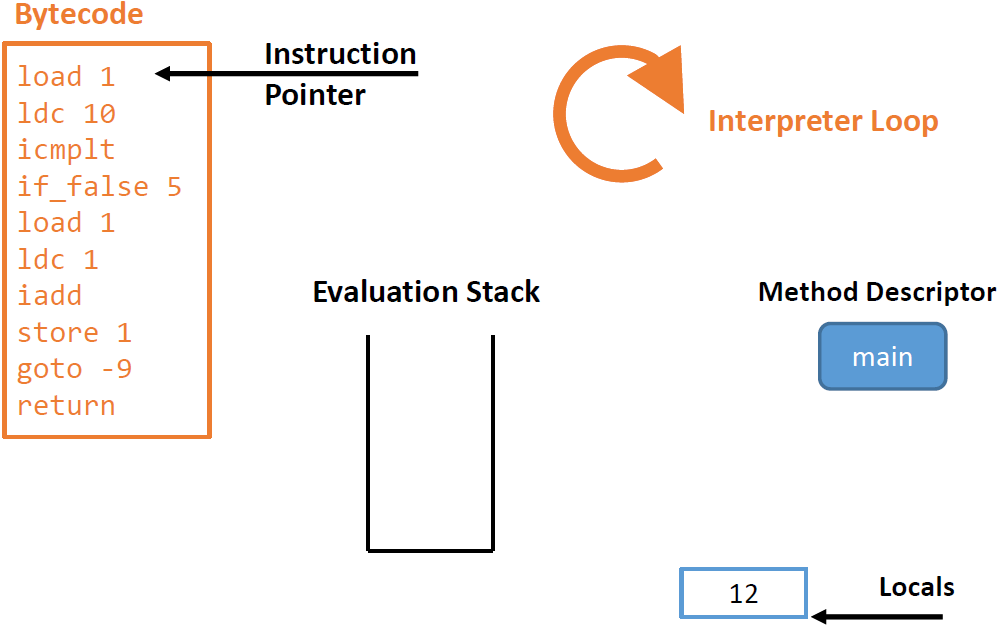
\includegraphics[width=0.7\linewidth]{interpreter.png}
\subsubsection{Bestandteile}
\textbf{Interpreter Loop}
\begin{itemize}
    \item Emuliert Instruktion nach der anderen
\end{itemize}
\textbf{Instruction Pointer (IP)}
\begin{itemize}
    \item Adresse der nächsten Instruktion
\end{itemize}
\textbf{Evaluation Stack}
\begin{itemize}
    \item Für virtuellen Stack Prozessor
\end{itemize}
\textbf{Locals \& Parameter}
\begin{itemize}
    \item Für aktive Methoden
\end{itemize}
\textbf{Method Deskriptor}
\begin{itemize}
    \item Für aktive Methode
\end{itemize}

\subsubsection{Implementation}
\begin{lstlisting}
private void execute(Instruction instruction) {
    var operand = instruction.getOperand();
    var frame = activeFrame();
    switch (instruction.getOpCode()) {
    case LDC -> push(operand);
    case ACONST_NULL -> push(null);
    case IADD -> {
        int right = checkInt(pop());
        int left = checkInt(pop());
        push(left + right);
    }
    // ISUB, IMUL, IDIV, IREM, INEG, BNEG
    case CMPEQ -> {
        var right = pop();
        var left = pop();
        if(left != null) {
            push(left.equals(right));
        } else {
            push(left == right);
        }
    }
    // CMPNE
    case ICMPLT -> {
        int right = checkInt(pop());
        int left = checkInt(pop());
        push(left < right);
    }
    // ICMPLE, ICMPGT, ICMPGE
    case IF_TRUE -> {
        if(checkBoolean(pop())) {
            frame.setInstructionPointer(frame.getInstructionPointer() + checkInt(operand));
        }
    }
    // IF\_FALSE
    case GOTO -> {
        frame.setInstructionPointer(frame.getInstructionPointer() + checkInt(operand));
    }
    case LOAD -> {
        push(getParamOrLocal(checkInt(operand))); 
    }
    case STORE -> {
        setParamOrLocal(checkInt(operand), pop());
    }
    case ALOAD -> {
        var arrayIndex = checkInt(pop());
        var pointer = checkPointer(pop());
        if(pointer == null) {
            throw new InvalidBytecodeException("Null pointer");
        }
        var length = heap.getArrayLength(pointer);
        if(arrayIndex < 0 || arrayIndex >= length) {
            throw new InvalidBytecodeException("Index out of bound");
        }
        var element = heap.readElement(pointer, arrayIndex);
        push(element);
    }
    // ASTORE
    case ARRAYLENGTH -> {
        var pointer = checkPointer(pop());
        if(pointer == null) {
            throw new InvalidBytecodeException("Null pointer");
        }
        push(heap.getArrayLength(pointer));
        
    }
    // GETFIELD
    case PUTFIELD -> {
        var field = checkFieldDescriptor(operand);
        var index = field.getIndex();
        var value = pop();
        checkType(value, field.getType());
        var instance = checkPointer(pop());
        if(instance == null) {
            throw new InvalidBytecodeException("Accessing uninitialized object");
        }
        heap.writeField(instance, index, value);
    }
    case NEW -> {
        var type = checkClassDescriptor(operand);
        var instance = newObject(type);
        push(instance);
    }
    case NEWARRAY -> {
        var length = checkInt(pop());
        if(length < 0) {
            throw new InvalidBytecodeException("Negative array size");
        }
        var descriptor = checkArrayDescriptor(operand);
        var pointer = heap.allocateArray(descriptor, length);
        for (int i = 0; i < length; i++) {
            heap.writeElement(pointer, i, defaultValue(descriptor.getElementType()));
        }
        push(pointer);
    }
    case INSTANCEOF -> instanceofTest(operand);
    case CHECKCAST -> checkCast(operand);
    case INVOKESTATIC -> invokeStatic(operand);
    case INVOKEVIRTUAL -> invokeVirtual(operand);
    case RETURN -> returnCall();
    default -> throw new InvalidBytecodeException("Unsupported instruction opcode");
    }
}
\end{lstlisting}

\subsubsection{Prozedurale Unterstützung}
\textbf{Methodenaufrufe}
\begin{itemize}
    \item invokevirtual: Aufruf neuer Methode
    \item return: Rücksprung aus Methode
\end{itemize}
\textbf{Activation Frame}
\begin{itemize}
    \item Datenraum einer Methode
    \item Parameter, lokale Variablen, temporäre Auswertungen
\end{itemize}
\textbf{Call Stack}
\begin{itemize}
    \item Stack der Activation Frames gemäss Aufrufreihenfolge
    \item Design:
    \begin{itemize}
        \item Managed im Interpreter: OO Darstellung für Komfort
        \item Unmanaged bei HW Execution: Kontinuierlicher Speicherblock für Effizienz
    \end{itemize}
\end{itemize}
\subsubsection{Gesamtbild}
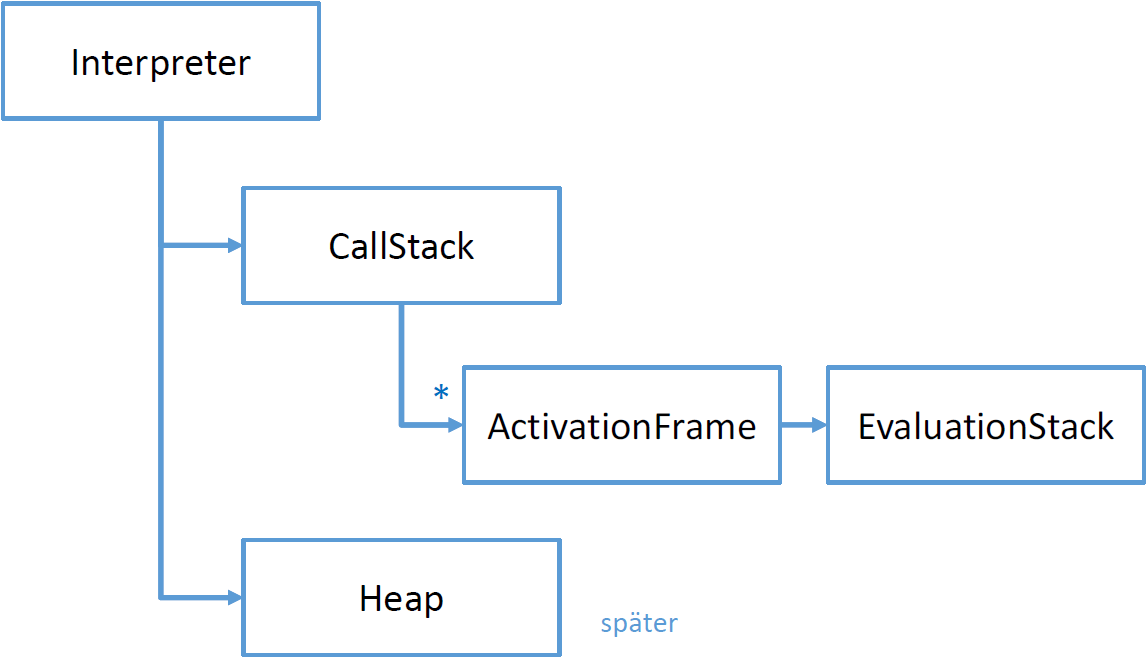
\includegraphics[width=0.5\linewidth]{gesamtbild.png}

\subsubsection{Verifikation im Interpreter}
\textbf{Korrekte Benutzung der Instruktionen}
\begin{itemize}
    \item Typen stimmen (e.g. \textit{checkInt()})
    \item Methodenaufrufe stimmen (Argumente, Rückgabe etc.)
    \item Sprünge sind gültig
    \item Op-Codes stimmen 
\end{itemize}

\subsubsection{Sicherheitsmassnahmen}
\begin{itemize}
    \item Korrekter Bytecode und Typkonsistenz prüfen
    \item Variablen immer initialisieren (auch lokale)
    \item Checks durchführen (Null, Array-Index etc.)
    \item Stack Overflow und Underflow Detection
\end{itemize}

\subsubsection{Interpretation vs. Kompilation}
\textbf{Interpreter ist ineffizient}
\begin{itemize}
    \item Dafür flexibel und einfach zu entwickeln
    \item Akzeptabel für selten ausgeführten Code
\end{itemize}
\textbf{Kompilierter HW-Prozessor Code ist schneller}
\begin{itemize}
    \item Just-In-Time (JIT) Compilation für Hot Spots
    \item Kompilation kostet, Laufzeit macht es (allenfalls) wett 
\end{itemize}